\documentclass[final,t,serif,mathserif]{beamer}

\mode<presentation>
{
  \usetheme{I6pd}
  \usefonttheme{professionalfonts}
}

% additional settings
\setbeamerfont{itemize}{size=\normalsize}
\setbeamerfont{itemize/enumerate body}{size=\normalsize}
\setbeamerfont{itemize/enumerate subbody}{size=\normalsize}

%\setbeamertemplate{bibliography item}[text]

% additional packages
\usepackage{times}
\usepackage{amsfonts}
\usepackage{amsmath, amssymb}
\usepackage{amsthm}
\usepackage{exscale}
\usepackage{algorithmic}
\usepackage{multicol}
%\boldmath
\usepackage{booktabs, array}
%\usepackage{rotating} %sideways environment
\usepackage[english]{babel}
\usepackage[latin1]{inputenc}
%\usepackage[orientation=landscape,size=a0,scale=1.3]{beamerposter}
\usepackage[orientation=landscape,size=custom,width=121,height=91,scale=1.5]{beamerposter}
%\usepackage[orientation=portrait,size=a4,scale=1.3]{beamerposter}
\listfiles
\usepackage{multicol}



% Display a grid to help align images
%\beamertemplategridbackground[1cm]


\newcommand{\h}{h}
\newcommand{\HK}{\mathcal{H}_K}
\newcommand{\f}{f}
\newcommand{\btheta}{g}
\newcommand{\bbartheta}{\boldsymbol{\bar{\theta}}}

\newcommand{\Risk}{\mathcal{R}}
\newcommand{\RiskLoss}{\mathcal{E}^{\ell}}
\newcommand{\Ltworho}{\mathcal{L}^2_{\rho_\fX}}
\newcommand{\Lonerho}{\mathcal{L}^1_{\rho_\fX}}
\newcommand{\frho}{f_\rho}
\newcommand{\flrho}{f^{\ell}_\rho}
\newcommand{\fcla}{f_c}
\newcommand{\fl}{f^{\ell}}
\newcommand{\flambda}{f_\lambda}

%\newcommand{\normK}[1]{\left\|{#1}\right\|_{\mathcal{H}_K}}
\newcommand{\normK}[1]{\left\|{#1}\right\|_K}
\newcommand{\normL}[1]{\left\|{#1}\right\|_{\Ltworho}}
\newcommand{\normLOne}[1]{\left\|{#1}\right\|_{\Lonerho}}

\newcommand{\bx}{\boldsymbol{x}}
\newcommand{\bX}{\boldsymbol{X}}
\newcommand{\bu}{\boldsymbol{u}}
\newcommand{\by}{\boldsymbol{y}}
\newcommand{\bY}{\boldsymbol{Y}}
\newcommand{\sY}{\mathcal{Y}}
\newcommand{\bhatY}{\boldsymbol{\hat{Y}}}
\newcommand{\bbary}{\boldsymbol{\bar{y}}}
\newcommand{\bbarv}{\boldsymbol{\bar{v}}}
\newcommand{\bz}{\boldsymbol{z}}
\newcommand{\bZ}{\boldsymbol{Z}}
\newcommand{\bphi}{\boldsymbol{\phi}}
\newcommand{\bbarphi}{\boldsymbol{\bar{\phi}}}
\newcommand{\bbaru}{\boldsymbol{\bar{u}}}
\newcommand{\bbarw}{\bar{f}}
\newcommand{\bbarZ}{\boldsymbol{\bar{Z}}}
\newcommand{\bbarz}{\boldsymbol{\bar{z}}}
\newcommand{\bhatZ}{\boldsymbol{\hat{Z}}}
\newcommand{\bhatz}{\boldsymbol{\hat{z}}}
\newcommand{\barz}{\bar{z}}
\newcommand{\bS}{\boldsymbol{S}}
\newcommand{\bbarS}{\boldsymbol{\bar{S}}}
\newcommand{\bc}{\boldsymbol{c}}
\newcommand{\ba}{\boldsymbol{a}}
\newcommand{\bw}{\boldsymbol{w}}
\newcommand{\bW}{\boldsymbol{W}}
\newcommand{\bU}{\boldsymbol{U}}
\newcommand{\bv}{\boldsymbol{v}}
\newcommand{\bzero}{\boldsymbol{0}}
\newcommand{\balpha}{\boldsymbol{\alpha}}
\newcommand{\sA}{\mathcal{A}}
\newcommand{\sC}{\mathcal{C}}
\newcommand{\sX}{\mathcal{X}}
\newcommand{\sS}{\mathcal{S}}
\newcommand{\sZ}{\mathcal{Z}}
\newcommand{\sbarZ}{\bar{\mathcal{Z}}}
\newcommand{\fbag}{\bold{F}}


\DeclareMathOperator*{\argmin}{arg\,min}
%\newcommand{\argmax}[1]{\underset{#1}{\operatorname{argmax}}}

\newcommand{\todo}[1]{\textcolor{red}{TODO: #1}}
\newcommand{\fixme}[1]{\textcolor{red}{FIXME: #1}}

\newcommand{\field}[1]{\mathbb{#1}}
\newcommand{\fY}{\field{Y}}
\newcommand{\fX}{\field{X}}
\newcommand{\fH}{\field{H}}

\newcommand{\R}{\field{R}}
\newcommand{\Nat}{\field{N}}
\newcommand{\E}{\field{E}}



\newcommand\theset[2]{ \left\{ {#1} \,:\, {#2} \right\} }
\newcommand\inn[2]{ \left\langle {#1} \,,\, {#2} \right\rangle }
\newcommand\RE[2]{ D\left({#1} \| {#2}\right) }
\newcommand\Ind[1]{ \left\{{#1}\right\} }
\newcommand{\norm}[1]{\left\|{#1}\right\|}
\newcommand{\diag}[1]{\mbox{\rm diag}\!\left\{{#1}\right\}}

\newcommand{\defeq}{\stackrel{\rm def}{=}}
\newcommand{\sgn}{\mbox{\sc sgn}}
\newcommand{\scI}{\mathcal{I}}
\newcommand{\scO}{\mathcal{O}}

\newcommand{\dt}{\displaystyle}
\renewcommand{\ss}{\subseteq}
\newcommand{\wh}{\widehat}
\newcommand{\ve}{\varepsilon}
\newcommand{\hlambda}{\wh{\lambda}}
\newcommand{\yhat}{\wh{y}}

\newcommand{\hDelta}{\wh{\Delta}}
\newcommand{\hdelta}{\wh{\delta}}
\newcommand{\spin}{\{-1,+1\}}

%\newcommand{\theHalgorithm}{\arabic{algorithm}}

% \newtheorem{lemma}{Lemma}
% \newtheorem{theorem}{Theorem}
% \newtheorem{cor}{Corollary}
% \newtheorem{remark}{Remark}
% \newtheorem{prop}{Proposition}

\newcommand{\reals}{\mathbb{R}}
\newcommand{\sign}{{\rm sign}}

\newcommand{\eg}{e.g.}
\newcommand{\ie}{i.e.}
\newcommand{\etal}{et al.}

\renewcommand{\P}{{\bf{P}}}

\newcommand{\textc}{\color{blue}}
\newcommand{\fgc}{\color{red}}
\newcommand{\othc}{\color{green}}
\newcommand{\bgc}{\color{black}}
\newcommand{\titc}{\bf\fgc}

\newcommand{\hY}{\widehat {Y}}
\newcommand{\hp}{\widehat {p}}

\newcommand{\sfrac}[2]{\mbox{$\frac{#1}{#2}$}}

\DeclareMathOperator*{\Exp}{\mathbf{E}}
\DeclareMathOperator{\Wealth}{Wealth}
\newcommand{\grad}{\nabla}
\renewcommand{\H}{\mathcal{H}}  % Hilbert space
\DeclareMathOperator{\Regret}{Regret}
\DeclareMathOperator{\polylog}{polylog}
\DeclareMathOperator{\Reward}{Reward}

\title{\huge Parameter-Free Convex Learning through Coin Betting}
\author{Francesco Orabona \and D\'avid P\'al}
\institute[] % (optional, but mostly needed)
{
  Yahoo Research, New York
}
\date[June 24, 2016]{June 24, 2016}

% abbreviations
\usepackage{xspace}
\makeatletter
\DeclareRobustCommand\onedot{\futurelet\@let@token\@onedot}
\def\@onedot{\ifx\@let@token.\else.\null\fi\xspace}
\def\eg{{e.g}\onedot} \def\Eg{{E.g}\onedot}
\def\ie{{i.e}\onedot} \def\Ie{{I.e}\onedot}
\def\cf{{c.f}\onedot} \def\Cf{{C.f}\onedot}
\def\etc{{etc}\onedot}
\def\vs{{vs}\onedot}
\def\wrt{w.r.t\onedot}
\def\dof{d.o.f\onedot}
\def\etal{{et al}\onedot}
\makeatother

\def\spazioBlocchi{\vspace{0cm}}
\def\spazio{\vspace{-0.325cm}}
\def\spazioo{\vspace{-0.3cm}}
\def\spaziooo{\vspace{-0.cm}}

%%%%%%%%%%%%%%%%%%%%%%%%%%%%%%%%%%%%%%%%%%%%%%%%%%%%%%%%%%%%%%%%%%%%%%%%%%%%%%%%%%%%%%%%%%%%%%%%%%%%%%%%%%%%
%%%%%%%%%%%%%%%%%%%%%%%%%%%%%%%%%%%%%%%%%%%%%%%%%%%%%%%%%%%%%%%%%%%%%%%%%%%%%%%%%%%%%%%%%%%%%%%%%%%%%%%%%%%%
\begin{document}
\begin{frame}{}

\begin{columns}[t]
  \begin{column}{.33\linewidth}

    \begin{block}{ARE YOU STILL TUNING HYPERPARAMETERS?}
      \spazio
      Regularized empirical risk objective
      \begin{equation}
      \label{equation:objective-function}
         \argmin_{w \in \R^d} \ \frac{\lambda}{2} \norm{w}^2 + \sum_{t=1}^N \ell(w, x_t, y_t)
      \end{equation}
      where $\ell$ is convex in $w$.
      \begin{itemize}
      \item Do you choose $\lambda$ manually?
      \item If you use SGD, how do choose the learning rate?
      \item Why is the algorithm not able to select $\lambda$ and learning rate automatically?
      \end{itemize}
      \spazio
    \end{block}


    \begin{block}{FROM COIN-BETTING TO MACHINE LEARNING}
    \spazio
    \begin{itemize}
      \item Problem~\eqref{equation:objective-function} can be solved with an Online Linear Learning algorithm.
      \item We prove that Online Linear Learning can be solved with online coin-betting algorithms.
    \end{itemize}

    \vspace{1cm}

    \begin{itemize}
      \item Coin flip outcome $c_t \in \{+1, -1\}$.
      \item You bet $|w_t|$ on the event $\sign(w_t) = c_t$, winning or losing $w_t c_t$.
      \item Krichevsky-Trofimov: Bet $\tfrac{1}{t} \sum_{i=1}^{t-1} c_i$ fraction of your current wealth
      \item \alert{KT algorithm for coin betting gives rise to optimal parameter-free algorithms for Online Learning, Convex Optimization and Machine Learning!}
      \item Key idea: Treat the gradient as the outcome of a coin flip.
      \item In other words: \alert{Learning rates are the results of suboptimal algorithms, they must be removed, not tuned/learned/adapted!}
    \end{itemize}
    \spazio
    \end{block}

    \begin{block}{THE HISTORY OF PARAMETER-FREE ALGORITHMS}
    %\begin{minipage}{.98\linewidth}
    \spazioo
    \begin{itemize}
    \item Streeter\&McMahan (2012): Regret in $\R^1$ that depends on $|u| \log|u|$ instead of $|u|^2$.
    \item Orabona (2013): Generalization to Hilbert space.
    \item McMahan\&Orabona (2014): Upper and lower bound $\norm{\bu} \sqrt{\log(\norm{\bu}+1)}$.
    \item Orabona (2014): Link between new online algorithms and self-tuning SVMs, and a data dependent bound.
    \item A parallel line of work on adaptive learning with expert advice: Chaudhuri et al. (2009), Chernov\&Vovk (2010), Luo\&Schapire (2014), Luo\&Schapire (2015), Koolen\&van-Erven (2015), Foster et al. (2015).
    \item Orabona\&P\'al (2016) proves that online adaptive algorithms for linear learning and learning with expert advices can be easily obtained from algorithms for coin-betting.
    \end{itemize}
    \spazioo

%     \begin{block}{BIBLIOGRAPHY}
%     \spazioo
%     %\vspace{-1cm}
%     %\begin{multicols}{2}
%     \tiny
%     Streeter and McMahan. No-regret algorithms for unconstrained online convex optimization. NIPS 2012.\\
%     Orabona. Dimension-free exponentiated gradient. NIPS 2013.\\
%     McMahan and Orabona. Unconstrained online linear learning in Hilbert spaces: Minimax algorithms and normal approximations. COLT 2014.\\
%     Orabona and Pal. From Coin Betting to Parameter-Free Online Learning. ArXiv 2016.
%     %\end{multicols}
%     %\vspace{-1cm}
%     \spazioo
%     \end{block}
%     \end{minipage}
    \end{block}


%     \begin{block}{UNCONSTRAINED ONLINE LEARNING WITH LIPSCHITZ LOSSES}
%     \spazioo
%     \centering
%     \begin{itemize}
%     \item Learning rate should be $\frac{\eta}{\sqrt{t}}$, e.g. Zinkevich (2003)
%     \item \alert{Setting $\eta$ optimally the regret is $\scO(\|\bu\| \sqrt{T})$ otherwise $\scO((\|\bu\|^2 +1)\sqrt{T})$}
%     \item Unfortunately the optimal $\eta$ depends on the \emph{future}
%     \end{itemize}
%     \begin{figure}
%       \includegraphics[width=15cm]{figs/cadata_keg_only}
%     \end{figure}
%     \spazioo
%     \end{block}

%     \begin{block}{EVEN MORE DETAILS: FOLLOW THE TIME-VARYING REGULARIZED LEADER}
%       \spazio
%       \begin{algorithmic}
% 	  \STATE{\bfseries Params:} A sequence of strongly convex functions $f_1,f_2,\dots$
%       % defined on a common domain $S \subseteq \fX$.
% 	  \STATE{\bfseries Initialize:} $\btheta_1=\boldsymbol{0}$
% 	  \FOR{$t=1,2,\dots$}
% 	  \STATE{Set $\bw_t=\nabla f_t^*(\btheta_t)= \arg \min_{\bw} f_t(\bw) - \langle \bw, \btheta_t \rangle$}
% 	  %\STATE{Set $\bw_t=\argmin_{\bw} f_t(\bw) - \langle \bw, \btheta_t \rangle = \nabla f_t^*(\btheta_t)$}
% 	  %\STATE{Observe $\bz_t$}
%           \STATE{Suffer loss $\ell_t(\bw_t)$}
% 	  \STATE{Update $\btheta_{t+1}=\btheta_{t} - \partial \ell_t(\bw_t)$}
% 	  \ENDFOR
%       \end{algorithmic}
%       \vspace{1cm}
%       \begin{itemize}
% 	\item Many names: FTRL (Cesa-Bianchi\&Lugosi, 2006); OMD (Shalev-Shwartz, PhD thesis 2007); RDA (Xiao, 2010)
% 	\item The ``regularizer'' is changing over time
% 	\item Not discarding any terms in the analysis!
%       \end{itemize}
%       \alert{Theorem.} \emph{
%       Assume $f_1,f_2,\dots$ such that each $f_t$ is $\beta_t$-strongly convex with respect to the norm $\norm{\cdot}_{f_t}$ (or $f^*_t$ $1/\beta_t$-strongly smooth). Then
%       \begin{equation*}
%       \sum_{t=1}^T \ell_t(\bw_t)  - \sum_{t=1}^T \ell_t(\bu)\leq f_T(\bu) + \sum_{t=1}^{T} \left(\frac{\bigl(\norm{\partial \ell_t(\bw_t)}_{f_t}\bigr)_*^2}{2 \beta_t} + f^*_t(\btheta_t)-f^*_{t-1}(\btheta_{t}) \right)~.
%       \end{equation*}
%       }
%       \spazio
%     \end{block}
%
%
%
%     \begin{block}{YET ANOTHER REGULARIZER}
%       \spazio
%       \begin{itemize}
%       \item $f_t(\bw)=\frac{\sqrt{t}}{\eta}\|\bw\|_2^2 \Rightarrow \text{ the bound is } \scO\left(\frac{\|\bu\|_2^2}{\eta}\sqrt{T} +\eta \sqrt{T} \right)$
%       \item What about $f_t(\bw)=\frac{\sqrt{t}}{\eta}\|\bw\|_2$? Not strongly convex!
%       \item We need something close but strongly convex, maybe we can add a logarithm...
%       \end{itemize}
%       \vspace{1cm}
%       \spazio
%     \end{block}


    \end{column}
    \begin{column}{.33\linewidth}

    \begin{block}{PARAMETER-FREE SGD BASED ON THE KT ESTIMATOR}
    \spazio
    %\begin{columns}[c]
      %\begin{column}{.7\linewidth}
	\begin{algorithmic}
	\STATE{Initialize $\Wealth_0 \leftarrow 1$ and $\theta_0 \leftarrow 0$}
	\FOR{$t=1,2,\dots,T$}
	\STATE{Set $w_t \leftarrow \Wealth_{t-1} \tfrac{\theta_{t-1}}{t} $}
	\STATE{Select an index $j$ at random from $\{1,2,\dots,N\}$}
	\STATE{Update $\theta_t \leftarrow \theta_{t-1} - \grad \ell(w_{t-1},x_j,y_j)$}
	\STATE{$\Wealth_t \leftarrow \Wealth_{t-1} - \langle \grad \ell(w_{t-1},x_j,y_j), w_t \rangle$}
	\ENDFOR
	\STATE{Output $\overline{w}_T = \tfrac{1}{T}\sum_{t=1}^T w_t$}
	\end{algorithmic}
      %\end{column}
      %\begin{column}{.3\linewidth}
%       \begin{itemize}
%       \item Parameter-free
%       \item Very easy to implement
%       \item Kernelizable
%       \item Same complexity of SGD
%       \end{itemize}
      %\end{column}
    %\end{columns}
    \spazio
    \end{block}

    \begin{block}{THEORETICAL GUARANTEES}
    \spazio
    The average $\overline{w}_T$ is an approximate minimizer of the objective \eqref{equation:objective-function}:
    \[
      \Exp\left[F(\overline{w}_T)\right] - F(\widehat{w}) \leq \tfrac{\norm{\widehat{w}}}{\sqrt{T}} \sqrt{\log(1+4 T^2 \norm{\widehat{w}}^2)} +\tfrac{1}{T} \; .
    \]
    \spazio
    \end{block}

    \begin{block}{DOES IT WORK FOR REAL?}
      \spazioo
      \begin{itemize}
        \item Split data into 75\% training + 25\% test
        \item Train with one pass over the training set and evaluate the final classifier on the test set.
        \item Use 5 different splits into training+test. Report average and standard deviation.
        \item We have run SGD with different learning rates and shown the performance of its last solution on the test set.
       \end{itemize}
      \begin{figure}[t]
	\centering
	\begin{tabular}{ccc}
	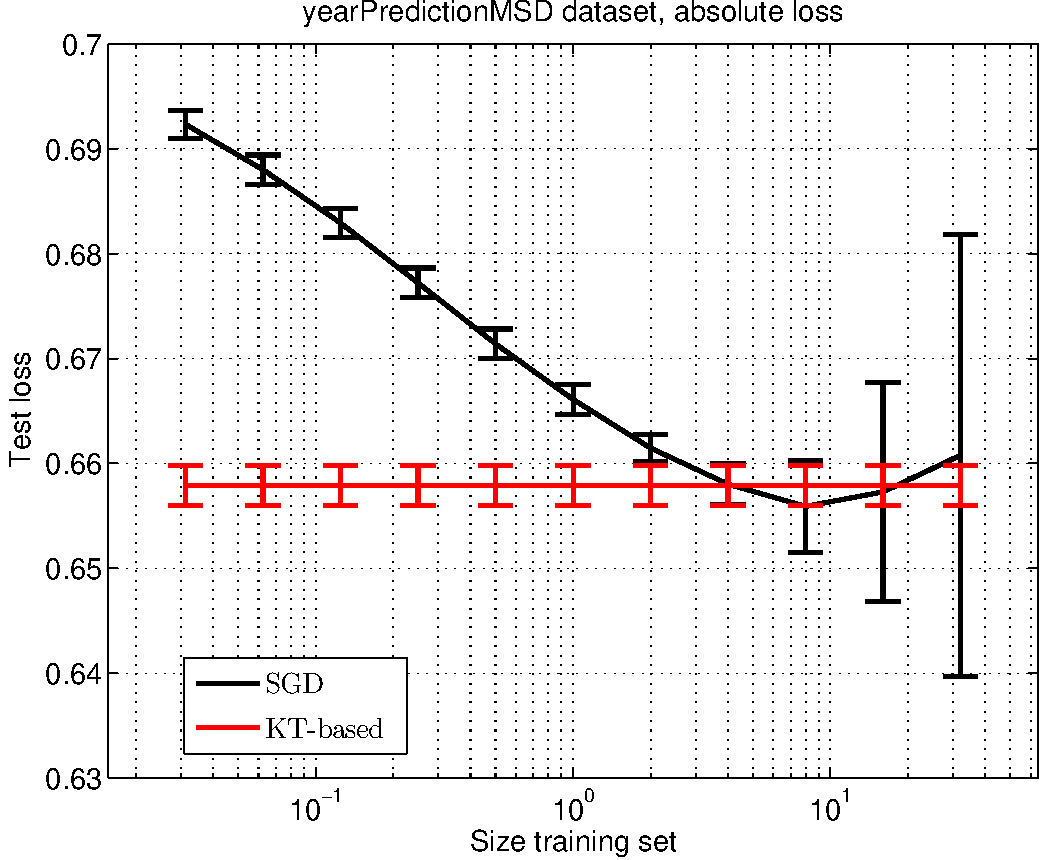
\includegraphics[width=0.32\textwidth]{../figs/yearPredictionMSD_kt_train_test-crop.pdf} &
        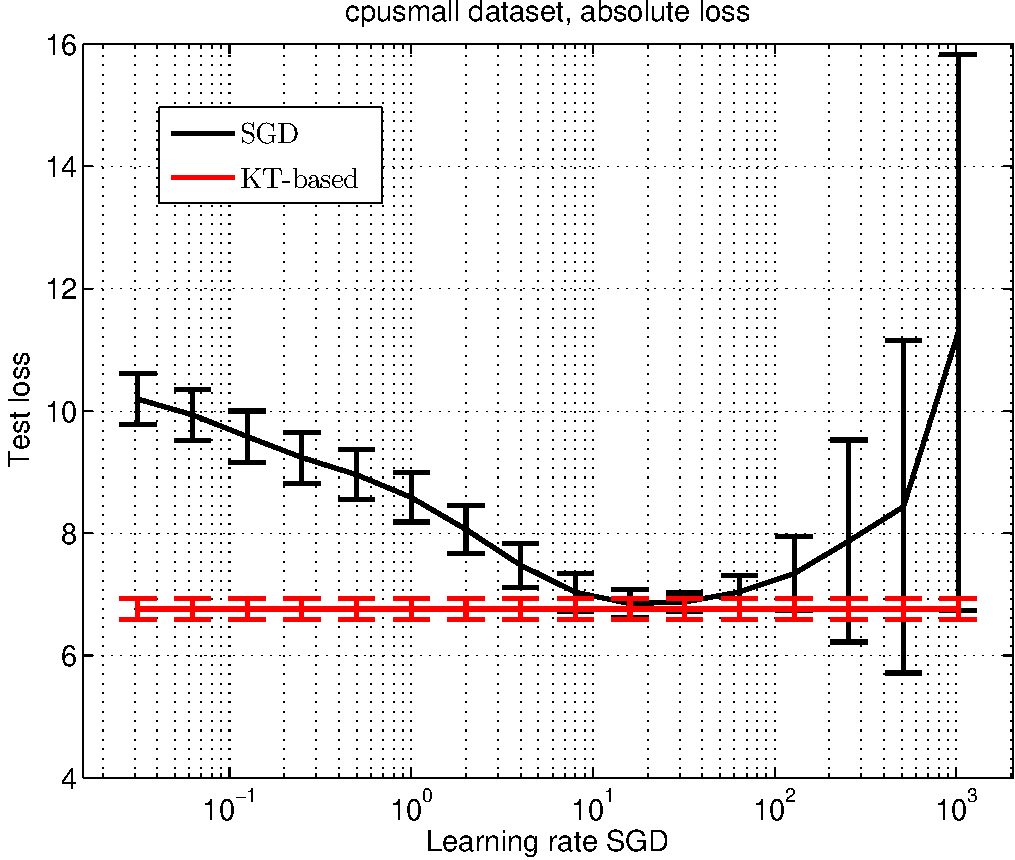
\includegraphics[width=0.32\textwidth]{../figs/cpusmall_kt_train_test-crop.pdf} &
        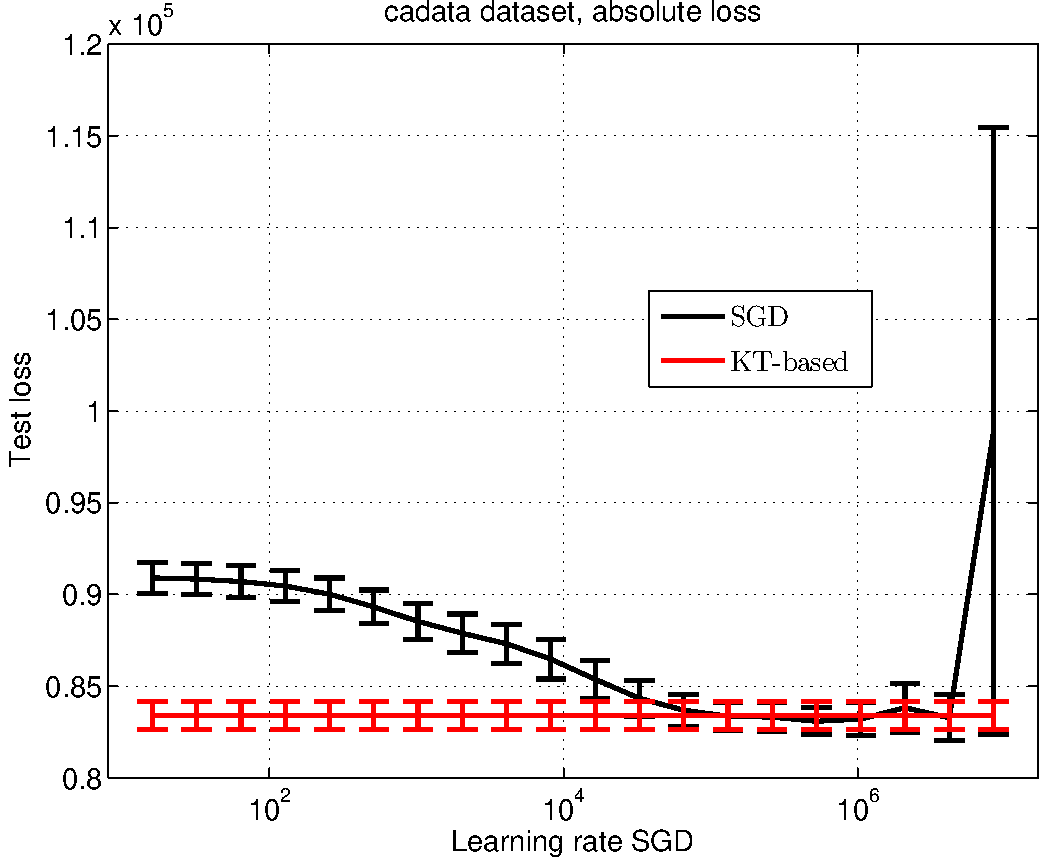
\includegraphics[width=0.32\textwidth]{../figs/cadata_kt_train_test-crop.pdf}
	\end{tabular}
      \end{figure}
      \begin{itemize}
        \item It is clear that the optimal learning rate is completely data-dependent.
        \item It is also interesting to note how the performance of SGD becomes very unstable with large learning rates. \item Yet \emph{our parameter-free algorithm has a performance very close to the unknown optimal tuning of the learning rate of SGD}.
       \end{itemize}
      \spazioo
    \end{block}


    \end{column}


    \begin{column}{.33\linewidth}


    \begin{block}{TECHNICAL DETAILS}
    \begin{minipage}{.98\linewidth}

    Read only if you want the math details!

    \begin{block}{LEARNING RATES IN ONLINE LINEAR LEARNING}
    \spaziooo
    \begin{itemize}
      \item Define
      \[
        \Regret_T(u) = \sum_{t=1}^T \langle \ell_t, w_t \rangle - \sum_{t=1}^T \langle \ell_t, u \rangle  \; .
      \]
      \item OGD with learning rate $\eta$ satisfies
	\[
	\forall u \in \H \qquad \Regret_T(u) \le \tfrac{\norm{u}^2}{2\eta} + \tfrac{\eta}{2} \sum_{t=1}^T \norm{\ell_t}^2
	\]
      \item Tons of algorithms adapt to the norms of the gradients, e.g. AdaGrad
      \item Adapting to the unknown norm of $u$ is \emph{more difficult and more important}.
      \item Better guarantees are indeed possible: Streeter\&McMahan (2012), Orabona (2013), McMahan\&Abernethy (2013), McMahan\&Orabona (2014), Orabona (2014) 
	\[
	\forall u \in \H \qquad \Regret_T(u) \le \big(O(1)+\polylog(1 + \norm{u})\norm{u} \big) \sqrt{T} \; .
	\]
    \end{itemize}
    \spaziooo
    \end{block}

    \begin{block}{REGRET GUARANTEE}
    \spaziooo
    \alert{Theorem.} \emph{
	Let $\{\ell_t\}_{t=1}^\infty$ be any sequence of loss vectors
	in a Hilbert space $\H$ such that $\norm{\ell_t} \le 1$.
	The KT-based online algorithm satisfies
	$$
	\forall \, T \ge 0, \
	\forall u \in \H \qquad
	\Regret_T(u) \le \norm{u} \sqrt{T \ln\left(1 + 4T^2 \norm{u}^2 \right)} + 1 \;.
	$$
    }

    \vspace{1cm}

    \alert{Proof Sketch.}
    \begin{itemize}
    \item Duality between wealth and regret: Let $F:\H \to \R$ be convex. For any $w_1, \dots, w_T$ and $g_1, \dots, g_T$,
    \[
      \underbrace{\sum_{t=1}^T \langle g_t, w_t \rangle}_{\Reward_T} \ge F\left( \sum_{t=1}^T g_t \right)
      \ \Leftrightarrow \
      \forall u \in \H, \
      \underbrace{\sum_{t=1}^T \langle g_t, u - w_t\rangle}_{\Regret_T(u)} \le F^*(u)
    \]
    \item Consider the $1$-dimensional case $\H=\R^1$.
    \item Set $w_t=\beta_t \Wealth_{t-1}$ where $\beta_t$ is the KT estimator.
    \item If $\ell_t \in \{+1, -1\}$, the results follows directly from the guarantee on the KT estimator and duality above.
    \item Extend to $\ell_t \in [-1,1]$ by convexity: The worst $\ell_t$ is always $+1$ or $-1$.
    \item Extend $1$-d case to Hilbert space: Worst direction is always parallel to the sum of the previous $\ell_t$.
    \end{itemize}
    \spaziooo
    \end{block}
    \end{minipage}
    \end{block}

  \end{column}
\end{columns}
\end{frame}
\end{document}
